\subsection{Prototype Performance Analysis}
\label{sec:prototype-performance}
To assist in identifying areas of improvement for the current prototype, preliminary testing has been undertaken using the OptiTrack system in the Extraterrestrial Environmental Simulation (EXTERRES) laboratory at The University of Adelaide. This testing will also form a baseline benchmark which can be compared to after algorithm implementation to conduct the validation and verification process outlined in Figure \ref{fig:systemsVdiagram}. The tests include using an adjustable ramp to measure the speed of the robot across different angles of incline and decline. The maximum incline and decline angles that the robot can travel can also be addressed. The ramp testing apparatus used for the preliminary testing in the EXTERRES laboratory is shown in Figure \ref{fig:testingappartus}. A mulit-terrain testing rig is also planned to be used to assess the robot's velocity and versatility on different terrains. The velocity of the robot will also be measured using the OptiTrack system to accurately assess gait effectiveness on different terrains. This testing has not yet occurred but is planned for the 30\textsuperscript{th} of May as shown in Appendix \ref{app:ganttChart}.

\begin{figure}[H]
    \centering
    \includegraphics[scale=0.13]{exterres_caveX_front.png}
    \caption{Preliminary testing of the CaveX robot using the incline rig in the EXTERRES laboratory.}
    \label{fig:testingappartus}
\end{figure}

\subsubsection{Incline and Decline Velocity Tests}
\label{sec:velocity-test}
The measurements for the robot's speed at different angles of incline and decline were taken for each of its three gaits: tripod, ripple, and wave. The inclination speed testing is shown in Figure \ref{fig:incline-velocity-test} and the MATLAB code used to process and plot the OptiTrack data is shown in Appendix \ref{app:MATLAB-code}.

\begin{figure}[H]
    \centering
    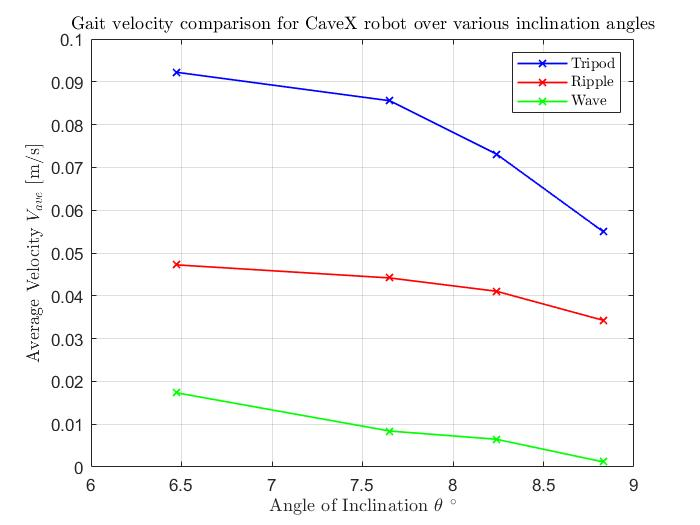
\includegraphics[scale=0.45]{Incline_velocity_tests.jpg}
    \caption{Gait velocity comparison of the CaveX robot for selected inclination angles}
    \label{fig:incline-velocity-test}
\end{figure}

The measurements in Figure \ref{fig:incline-velocity-test} show that as the angle of inclination increases, the speed of the robot decreases. Further, they show an inverse relation between static stability and velocity. The tripod gait has the highest speed of the three gaits but it reduces sharply as the angle increases. The ripple gait is the second fastest and appears to have a slight decrease in speed as angle increases. Lastly, the wave gait has the slowest speed measured. As the angle increases to the last measured angle of 8.83\textdegree, the speed of the wave gait approaches a zero value which represents the angle that the robot can no longer traverse the ramp. The decreasing trend in speed between the gaits also follows a concordant decrease in the number of moving legs. Thus, it is likely that the reason for such change is a reduced net force applied to the robot. The speed measurements for the decline testing across each of its three gaits is shown in Figure \ref{fig:decline-velocity-test}.

\begin{figure}[H]
    \centering
    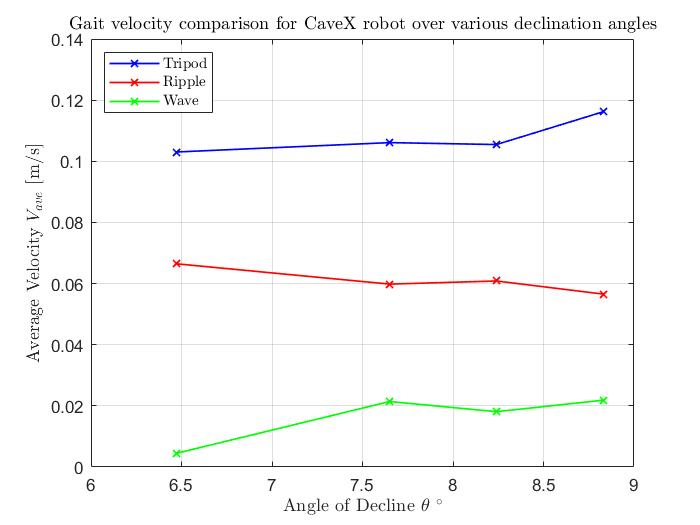
\includegraphics[scale=0.45]{Decline_velocity_tests.jpg}
    \caption{Gait velocity comparison of the CaveX robot for selected declination angles}
    \label{fig:decline-velocity-test}
\end{figure}

The results in Figure \ref{fig:decline-velocity-test} show that the tripod gait has the fastest movement speed across the decline angles, similar to the results shown in Figure \ref{fig:incline-velocity-test}. As the angle of declination is increased, the speed of the robot in its tripod gait increases. The ripple gait is again the second fastest gait. However, as the declination angle is increased its speed slightly decreases. Lastly, the wave gait is the slowest gait. As the declination angle increases the speed appears to increase. A noteworthy observation is that the change in speed between decline angles is relatively small compared to the inclined tests.

\subsubsection{Summary}
The testing results show consistency between the fastest and slowest gaits. The incline speed testing results demonstrate that the speed of the prototype decreases as the slope increases, an expected trend as the robot must overcome a larger vertical component of its own weight as the angle increases. In the declination results, the speed is observed to increase for the tripod and waves gaits but slightly decrease for the ripple gait. The difference in the trend of the results across the three gaits in the declination testing is due to the difference in stability and leg movements. This means that some gaits, such as the tripod and wave, are better suited to a declined slope as they allow for faster movement. The ripple gait is less impacted by the incline and decline angles as observable by the shallower slopes shown in the figures.